\documentclass[11pt]{article}

% --- Packages ---
\usepackage[utf8]{inputenc}
\usepackage{geometry}
\geometry{letterpaper, margin=1in}
\usepackage{graphicx}
\usepackage{booktabs}
\usepackage[hidelinks]{hyperref}
\usepackage{amsmath}
\usepackage{caption}
\usepackage{float}
\usepackage{setspace}
\usepackage{xcolor}
\usepackage{listings}

% --- Code Listing Style ---
\definecolor{codegreen}{rgb}{0,0.6,0}
\definecolor{codegray}{rgb}{0.5,0.5,0.5}
\definecolor{codepurple}{rgb}{0.58,0,0.82}
\definecolor{backcolour}{rgb}{0.95,0.95,0.92}

\lstdefinestyle{pystyle}{
    backgroundcolor=\color{backcolour},   
    commentstyle=\color{codegreen},
    keywordstyle=\color{magenta},
    numberstyle=\tiny\color{codegray},
    stringstyle=\color{codepurple},
    basicstyle=\ttfamily\footnotesize,
    breakatwhitespace=false,         
    breaklines=true,                 
    captionpos=b,                    
    keepspaces=true,                 
    numbers=left,                    
    numbersep=5pt,                  
    showspaces=false,                
    showstringspaces=false,
    showtabs=false,                  
    tabsize=2
}
\lstset{style=pystyle}

% Academic spacing
\onehalfspacing

\title{\textbf{Tracked: Analyzing and Predicting Amtrak Train Delays}}
\author{\textbf{STA 220 Project} \\ \textbf{Subhadithya, Vikhas, Pavan, Rithvik} \\ \textit{Data Engineering and Machine Learning Pipeline} \\ \vspace{0.1cm} \href{https://github.com/pavan-nuthi/Amtrak-delay-analyzer}{\texttt{github.com/pavan-nuthi/Amtrak-delay-analyzer}}}
\date{}

\begin{document}

\pagenumbering{arabic}
\setcounter{page}{1}
\maketitle

\vspace{1cm}
\section{Abstract}

The train schedules in the United States usually have a lot of unpredictable delays, and this leads to inefficient connectivity, and people fear taking the trains for this reason. This project mainly focuses on Amtrak delays and figuring out the factors that really affect them, and verifying whether a machine learning algorithm can reliably forecast them. We designed an end-to-end data collection pipeline that scraped over 2.3 million real-time data points from the amtraker api, and we combined this data with geographical metadata and weather data for the major stations. We then cleaned it down to approximately 1021244 data points and used this data for training and testing the machine learning model.

The conclusions demonstrate that weather data, which has parameters like maximum wind speed, maximum temperature, and precipitation, shows very minimal effect in deciding delays, and most people assume that bad weather plays a major role, but our correlation did not support that. Also, the ANOVA analysis showcased route-level and geographic factors as the most determining factors in deciding the delay. To go further with prediction, we trained a Random Forest model using these features, achieving an $R^2$ of 0.78 and MAE of $\sim$7.0. This report walks through the architecture, implementation, and data analysis used for predicting the delays, and our model can forecast the delays for future days by consuming real-time data.

\clearpage

\section{Introduction}

\subsection{Motivation and Problem Statement}

In United States, Amtrak is considered to be one of the biggest intercity passenger rail system and runs with constant delays at all times. This mainly affects travellers and makes the logistics very tough and also increases the operational expenses.
A common societal assumption considers severe weather phenomena to be the primary catalyst causing these transit gridlocks. The distinct goal of this research project is dual-fold: First, to statistically investigate whether environmental occurrences (weather) or systemic network constraints (infrastructure) drive prolonged delays. Second, to operationalize these findings into a programmatic machine learning model capable of accurately forecasting delay outcomes mathematically based on localized and real-time conditions relative to track progression.



\subsection{Dataset Sources, Variables, and Size}
In order to collect the historical dataset required for real-time prediction of delays, we noted that Amtrak only publishes real-time data as open source. Therefore, we used our cron job script to run periodically (approximately 96 times per day), collecting over 2.3 million records over a window of two weeks. We used the below API to further extend the features of the data.
\begin{itemize}
   \item \textbf{Amtraker API v3 \cite{ref:amtraker}:} Continuously queried to intercept JSON payloads detailing live track coordinates, velocity, and scheduled versus actual arrival matrices for active units.
    \item \textbf{Wikipedia HTML Tables \cite{ref:wiki}:} Extracted via \texttt{BeautifulSoup} to scrape unlisted station metadata (City and State/Province), subsequently cross-referenced with 3-letter Amtraker API station codes.
    \item \textbf{Open-Meteo API \cite{ref:meteo}:} Queried to collect historical, high-resolution daily weather metrics (inclusive of maximum wind speed, precipitation sum, and temperature variations). Given rate-limit constraints, queries were bound strictly to the coordinates of 10 primary tier-one transit hubs across the continent..
\end{itemize}

\subsection{Hypotheses and Research Questions}
We formalized three dominant Research Questions (RQs):
\begin{enumerate}
    \item \textbf{RQ1:} What are the most and least delayed routes in the Amtrak network, and how do they accumulate delay linearly over a journey?
    \item \textbf{RQ2:} Is there a strong statistical correlation between extreme weather events (wind, precipitation) and severe train delays?
    \item \textbf{RQ3:} Can an ensemble machine learning architecture effectively predict real-time delay minutes relying solely on derived API factors?
\end{enumerate}
We initially hypothesized noticeable delay variations dictated by cross-country routes and expected a relatively strong positive correlation between adverse weather strings and transit halts.

\section{Methods}


\begin{figure}[H]
    \centering
    \includegraphics[width=0.75\textwidth]{image.png}
    \caption{End-to-end architecture of the automated data pipeline with real-time API scraping, SQLite storage, and machine learning deployment.}
    \label{fig:architecture}
\end{figure}

As illustrated in Figure \ref{fig:architecture}, the project executes through a seamless, automated three-level architecture:
\begin{enumerate}
    \item \textbf{Data Ingestion Layer:} A Python \texttt{cron} tracker routinely executes data pulls from the Amtraker API (live logistics), Wikipedia (station metadata), and Open-Meteo (hub weather thresholds).
    \item \textbf{Relational Storage:} Extracted JSON arrays and HTML strings are normalized into a persistent SQLite database, securing data inside linked \texttt{routes}, \texttt{stations}, and \texttt{delay\_logs} tables to prevent duplication boundaries over extended deployment.
    \item \textbf{Analytical Modeling:} Local Jupyter environments execute native statistical functions, mapping SQL endpoints dynamically to render structural EDA grids, test associative hypotheses, and orchestrate the Random Forest prediction frameworks directly against continuous data. 
\end{enumerate}

\subsection{Data Acquisition and Storage}
For the data pipeline it was necessary to maintain the stateless requests against the API. At the same time it was also required to aggressively prevent duplicate logs which were being generated due to the querying of the same active train multiples times in an hour. We used SQLite relational database which used primarily three entities:  \texttt{routes}, \texttt{stations}, and \texttt{delay\_logs}. 

 We actively supressed the generation of duplicate record by utilizing SQL \texttt{UPSERT} procedures- the timestamps were updated if there was occurence of similar \texttt{station\_code} trigger or by the insertion of new entities as they spawned . 

\begin{lstlisting}[language=SQL, caption=Example of the UPSERT architecture utilized during real-time data scraping]
INSERT INTO delay_logs (
    scrape_time, train_number, train_id, route_name,
    station_code, station_name, scheduled_arrival, 
    actual_arrival, delay_arrival_min, status
) VALUES (?, ?, ?, ?, ?, ?, ?, ?, ?, 'Departed')
ON CONFLICT(train_id, station_code) DO UPDATE SET
    actual_arrival = excluded.actual_arrival,
    delay_arrival_min = excluded.delay_arrival_min;
\end{lstlisting}

\subsection{Cleaning and Feature Engineering}
We needed to rigorously sanitize the unrefined dataset. To constrict focus onto the US domestic network Canadian VIA routes were strategically filtered from the dataset. Additionally, to detect errors grom API logical checks were used. We removed unrealistic timestamp changes for which the resulting delay produced was more than 500 hours. These were removed as it was usually caused by inactive API endpoints which still tracked parked units. After the conclusion of the data cleaning process we were left with 1021244 valid data points. 

For feature engineering we mainly focussed on the topological and chronological factors.  Engineering of \texttt{delay\_arrival\_min} was done by the extraction of differentials seconds between ISO 8601 strings. We used Pandas \texttt{dt} accesor in order to generate chronological variables (\texttt{Hour\_of\_Day}, \texttt{Day\_of\_Week},  \texttt{Is\_Weekend}). From the perspective of the network structure to isolate the transit progression, the window function queried the  \texttt{delay\_logs} and grouped the \texttt{train\_id}. The index was mapped to a explicitly new \texttt{Stop\_Number} feature. Subsequently for structural matrix adherence the features were label encoded.

\subsection{Statistical Analysis Models}
To address RQ1 i.e. system delays the delay changes over time was visualized using EDA or exploratory data analysis. We used ANOVA (One-Way Analysis of Variance) to make sure there was statistical robustness. Significant F-statistics were identified. This was done by designating route strings as factors against the numerical variable. To compare the numerical weather data and delay values Pearson's $r$ and Spearman's  $\rho$ tests were used. This was done to study the correlations (RQ2).

\subsection{Machine Learning Optimization}
Gradient Boosting Regressors were compared to Random Forest architectures by the analytical models in order to synthesize network variables mathematically (RQ3). The reason for choosing Random Forest as the best model was because complex, nonlinear patterns can be handled naturally by its group of decision trees. For example, increase in delay does not happen in a simple way- if a freight schedule window is missed a 5 minute delay will grow into half an hour. 80/20 partitioning were explicitly used for Train-to-Test distribution.


\section{Results}

\subsection{Network Variances and Temporal Analysis}

\subsubsection{Exploratory Delay Patterns by Route}
Vast disparities linked specifically to specific train routes were quickly discovered by the investigation of the baseline transit efficiency. Strong logical blocks were implied by average  \texttt{delay\_arrival\_min} aggregates by utilizing the flattened dataset. These strong logical blocks were innate to bigger intercontinental tracks (such as the \textit{Sunset Limited} or \textit{California Zephyr}) relative to urban commuting paths which were comparatively tighter (e.g., \textit{Northeast Regional}).

\begin{figure}[H]
    \centering
    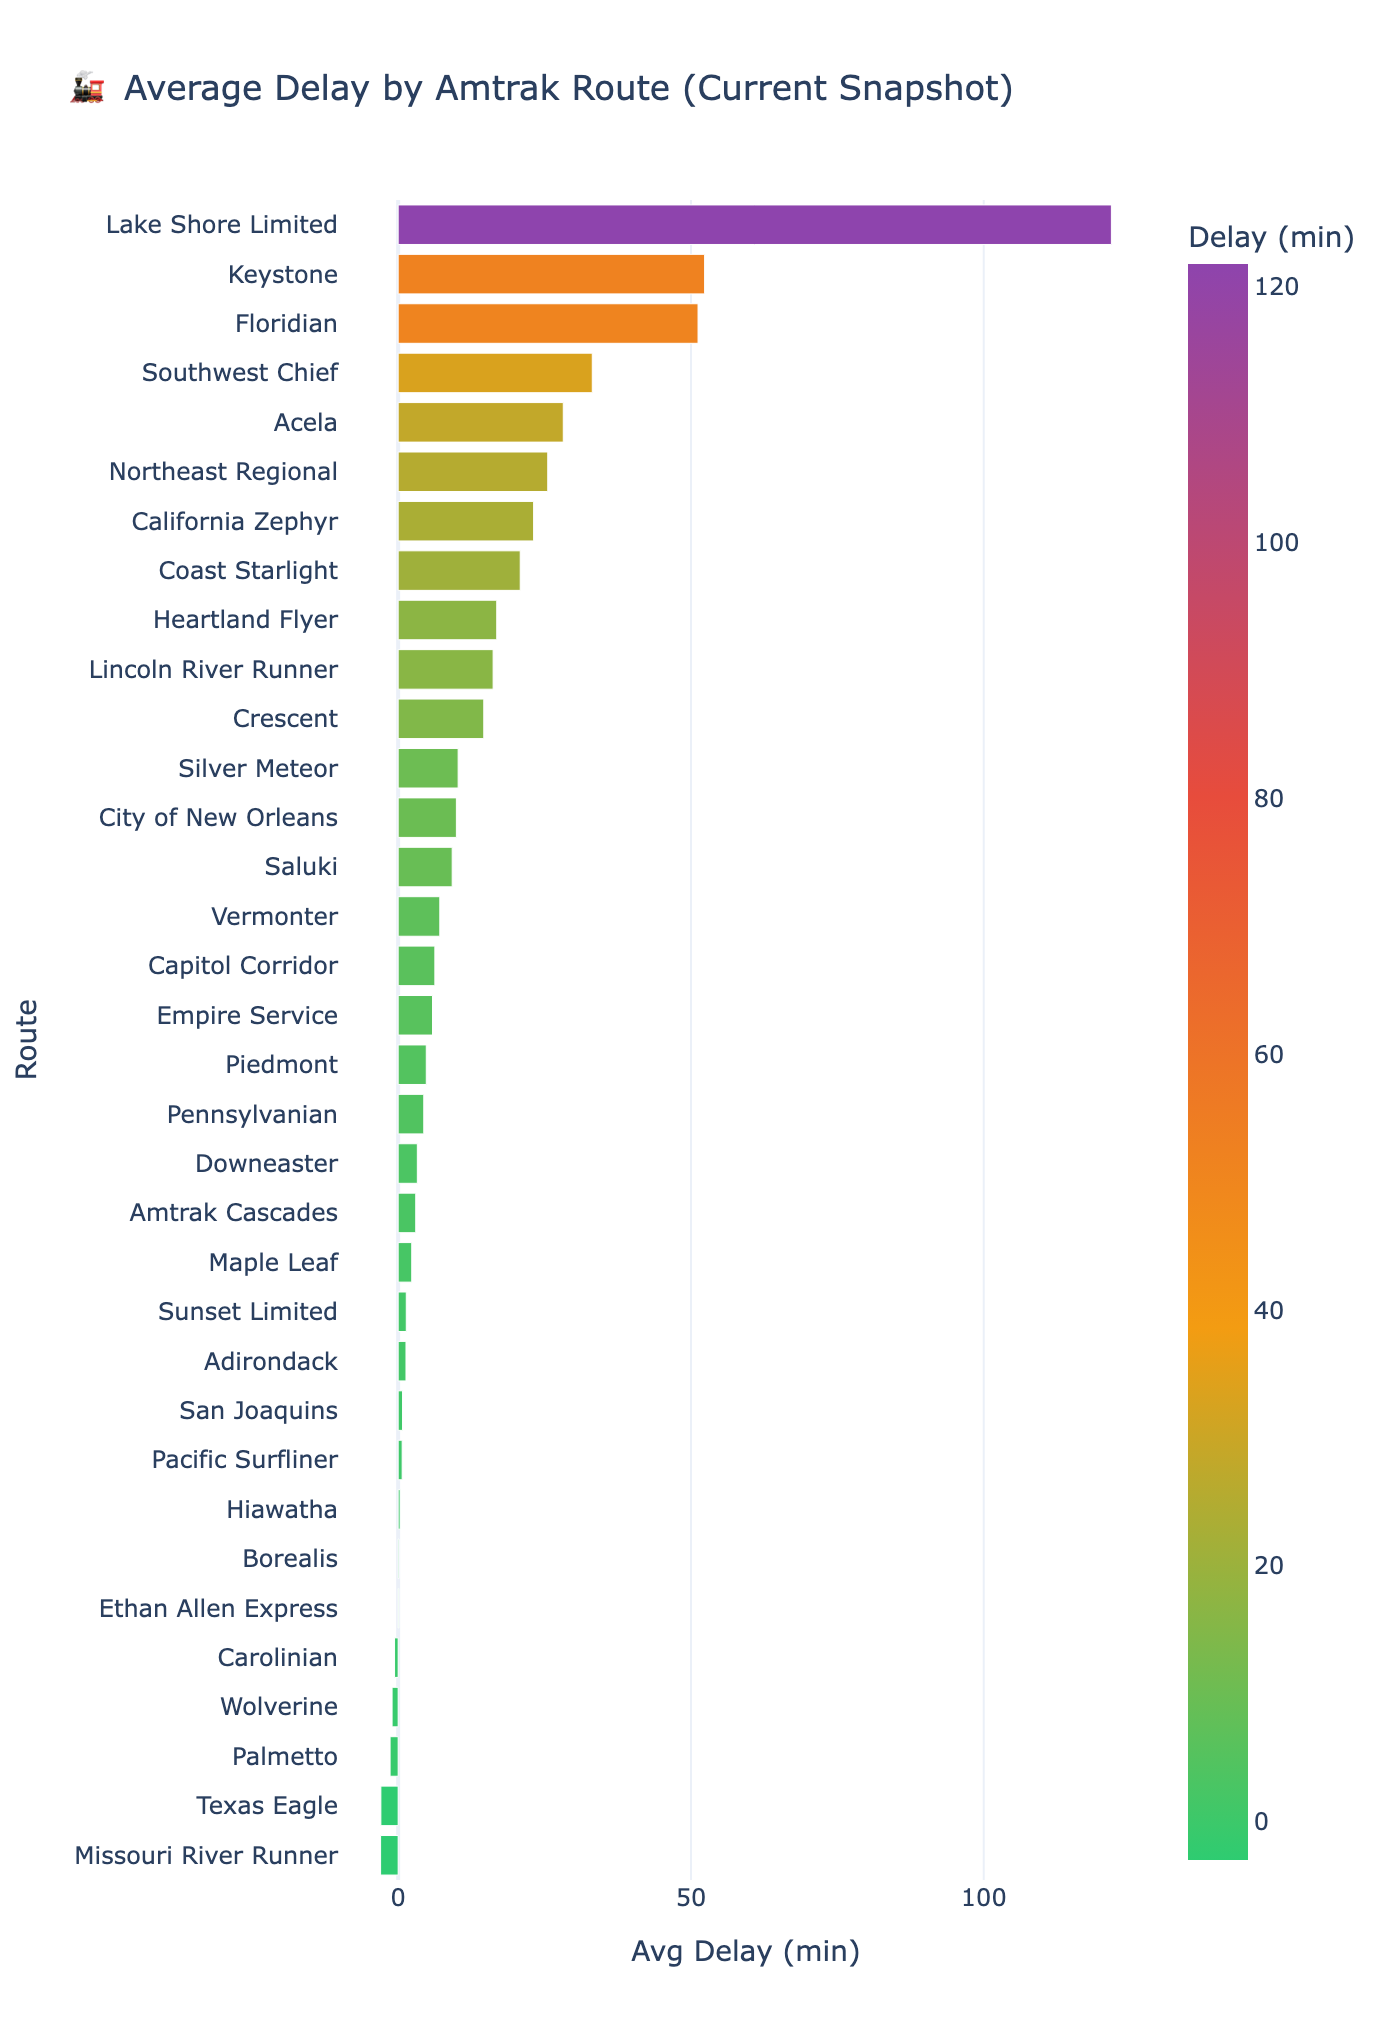
\includegraphics[width=0.65\textwidth]{delay_by_route.png}
    \caption{Average Arrival Delay by Amtrak Route. Visualizes the disparate baseline lag indicating systemic infrastructure blocks dependent upon route geography.}
    \label{fig:routes}
\end{figure}

To dynamically reinforce the observations' statistical foundation we utilized a One-Way ANOVA across 34 discrete routes. After the analysis of 1,100 active observations, the test spitted out a significant F-statistic of 9.30  along with a $p$-value which was mathematically approximately 0.000 ($p < 0.05$). This resulted in the rejection of the null hypothesis and a conclusion was reached that the origin of the route and the way in which the tracks are shared strongly influences the delays.

\begin{table}[H]
    \centering
    \caption{One-Way ANOVA: Delay Differences Across Routes}
    \vspace{0.2cm}
    \begin{tabular}{@{}lc@{}}
        \toprule
        \textbf{Metric} & \textbf{Value} \\
        \midrule
        Number of Routes Tested & 34 \\
        Total Observations & 1100 \\
        F-Statistic & 9.3013 \\
        $p$-value & $< 0.001$ \\
        Significance Level ($\alpha$) & 0.05 \\
        Reject Null Hypothesis ($H_0$) & Yes \\
        \bottomrule
    \end{tabular}
    \label{tab:anova_stats}
\end{table}

\subsubsection{Chronological Congestion}
A proper pattern can be observed when the delays were plotted over the course of the day. Predicted structural clustering can be seen during expected high-traffic gridlock hours and evening cascade points.

\begin{figure}[H]
    \centering
    \begin{minipage}{0.48\textwidth}
        \centering
        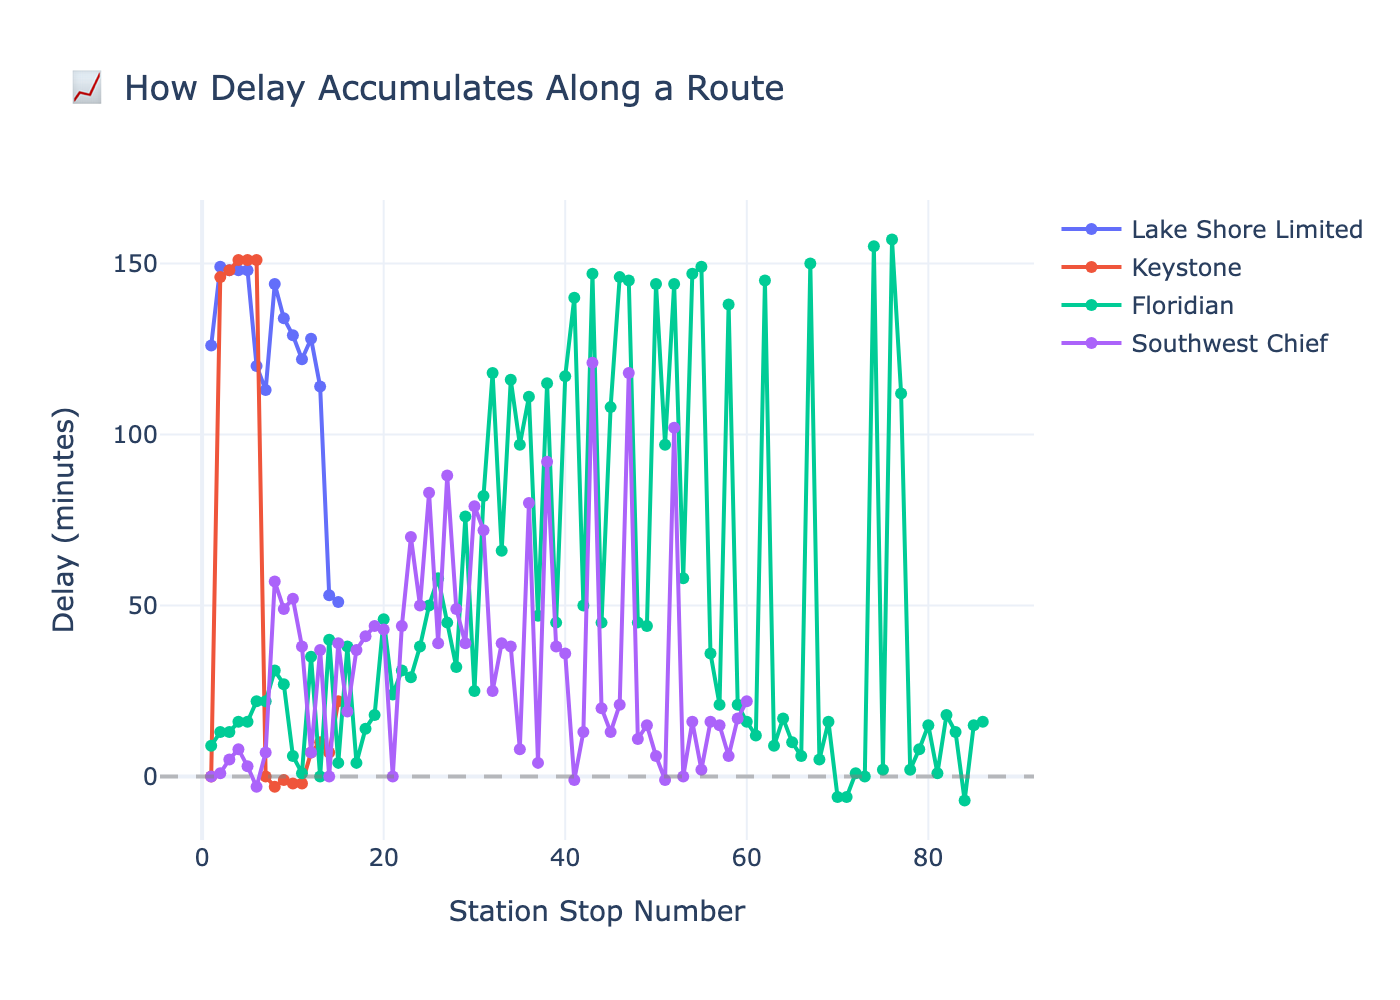
\includegraphics[width=\linewidth]{delay_accumulation.png}
        \caption{Rolling chronological delay accumulation}
    \end{minipage}\hfill
    \begin{minipage}{0.48\textwidth}
        \centering
        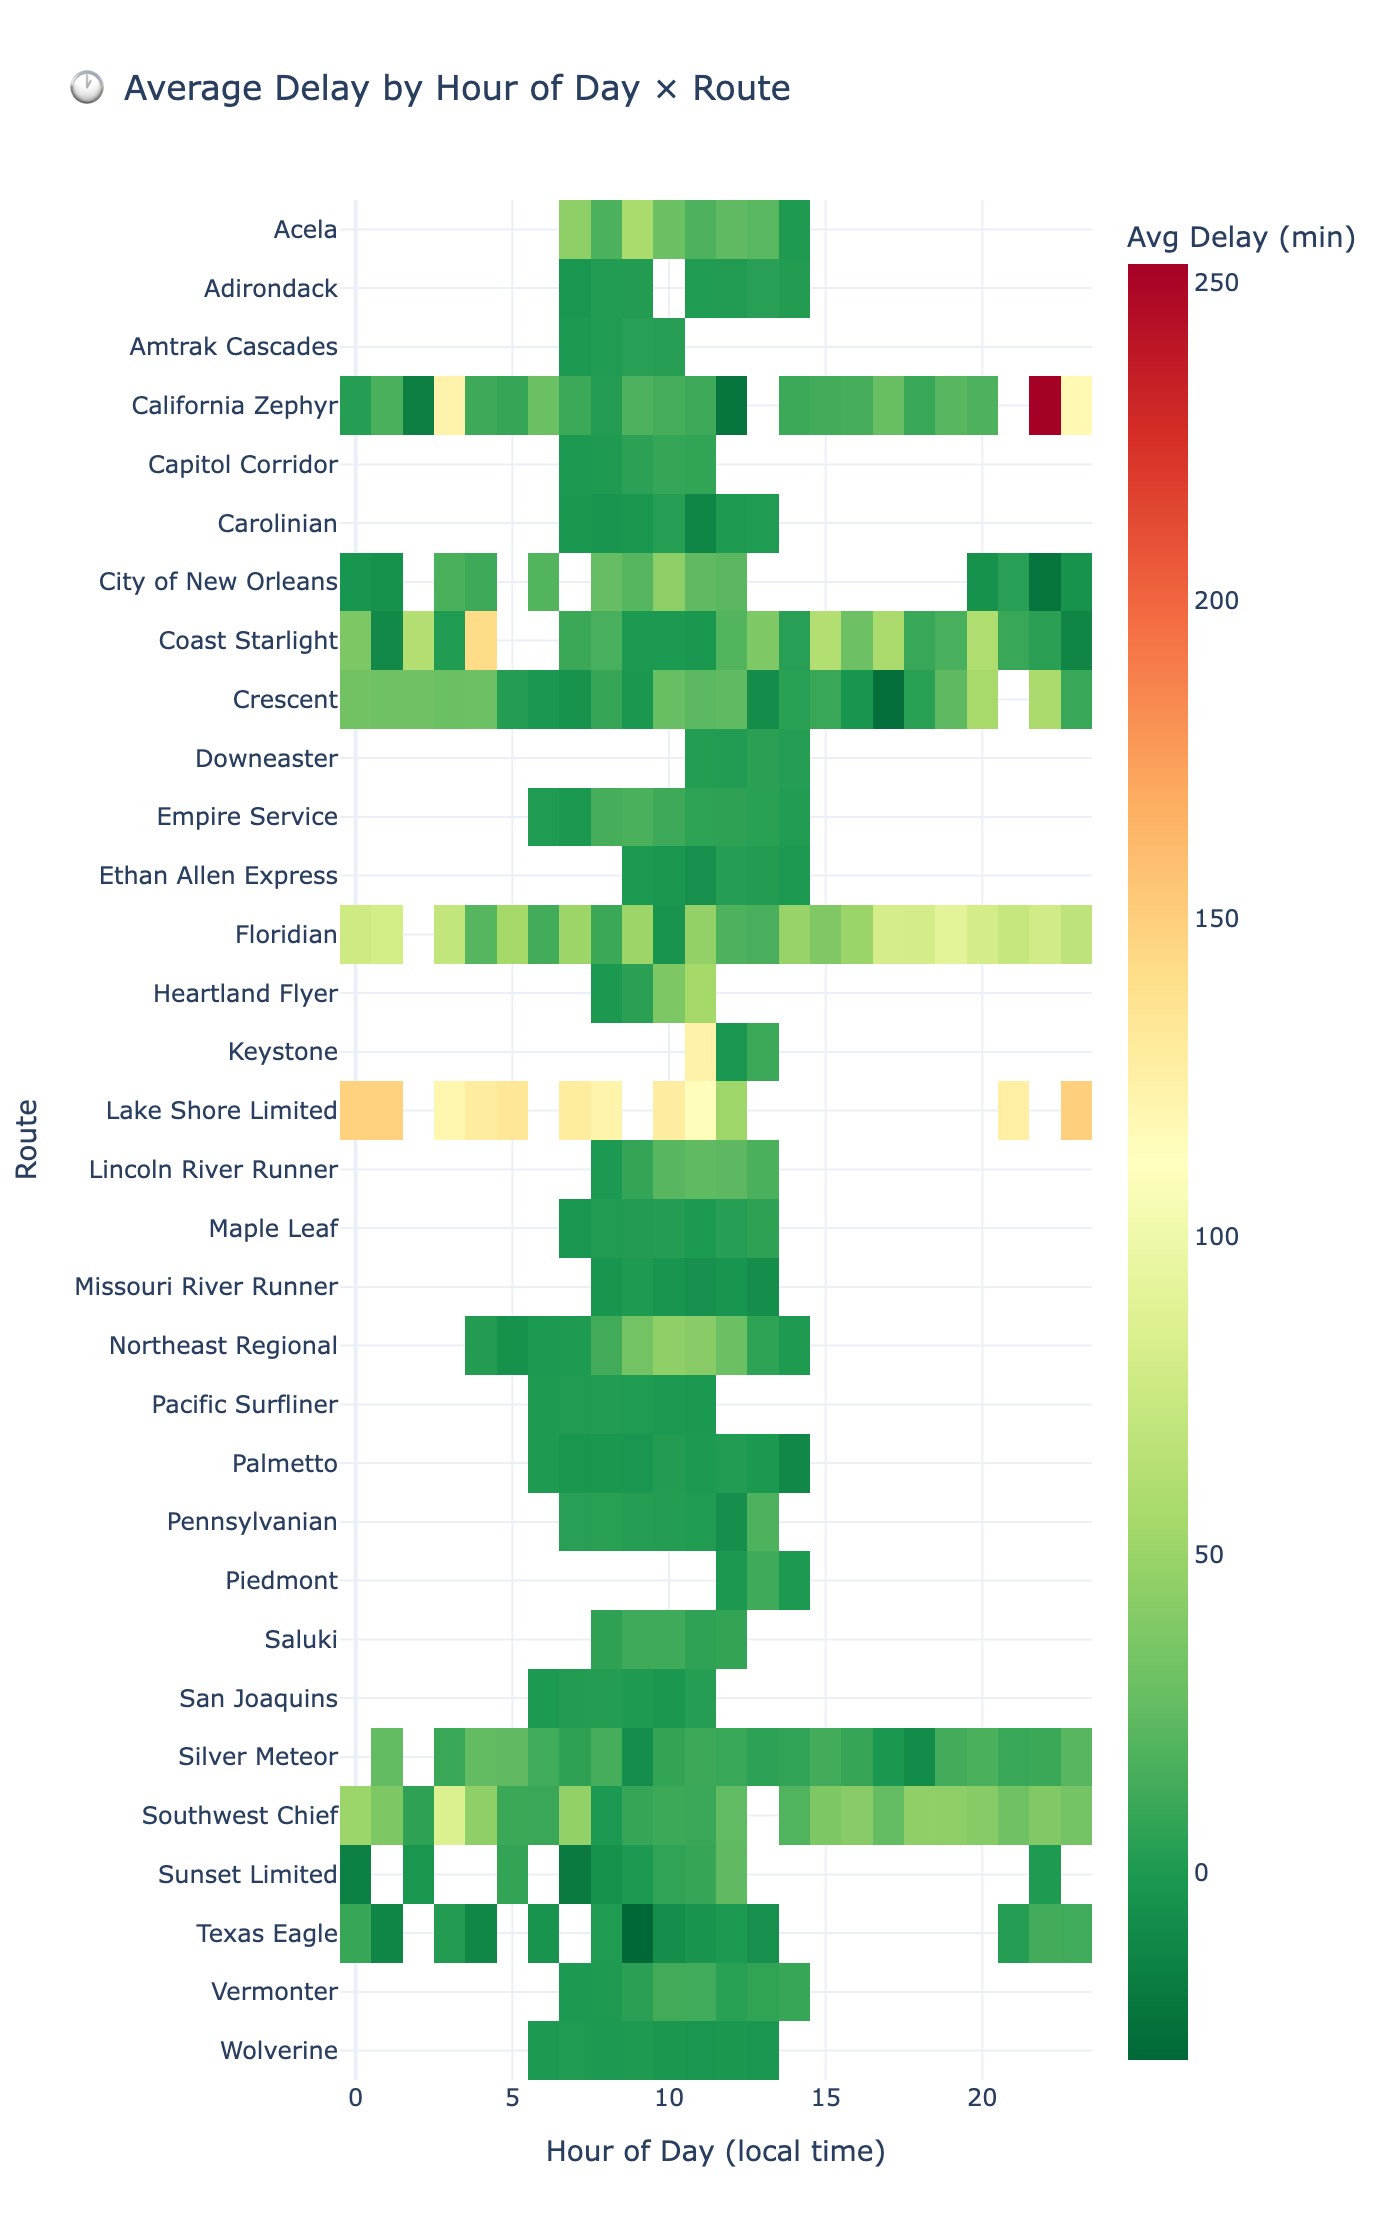
\includegraphics[width=\linewidth]{delay_by_hour_route.png}
        \caption{Violin distribution of delays per hour blocks}
    \end{minipage}
\end{figure}

\subsection{Meteorological and Weather Correlation}

\subsubsection{Visual Scatter Testing}
Many people assume that the weather might be a primary reason for the delay of trains. To check this we get the weather data of 10 major hubs across the USA (Los Angeles, Sacramento, New York, etc.) to test these hypotheses. We get the temperature, precipitation, and wind data in these 10 major hubs and compare the current day delay with the delays of the previous seven days. The scatter plot (Figure \ref{fig:scatter}) shows the delays  of the trains across varying precipitation and wind weather conditions

The plots visually reveal no trends. The severe delays, ranging from 40 to 80 minutes, cluster near the zero bound of the precipitation axis and within moderate wind speeds (10 to 30 km/h). These scatter plots provide evidence that train delays might occur even during clear days, proving that the delays happen independently of any environmental issues. The delays might be due to other factors, like freight train delays and congestion patterns in major cities.

\begin{figure}[H]
    \centering
    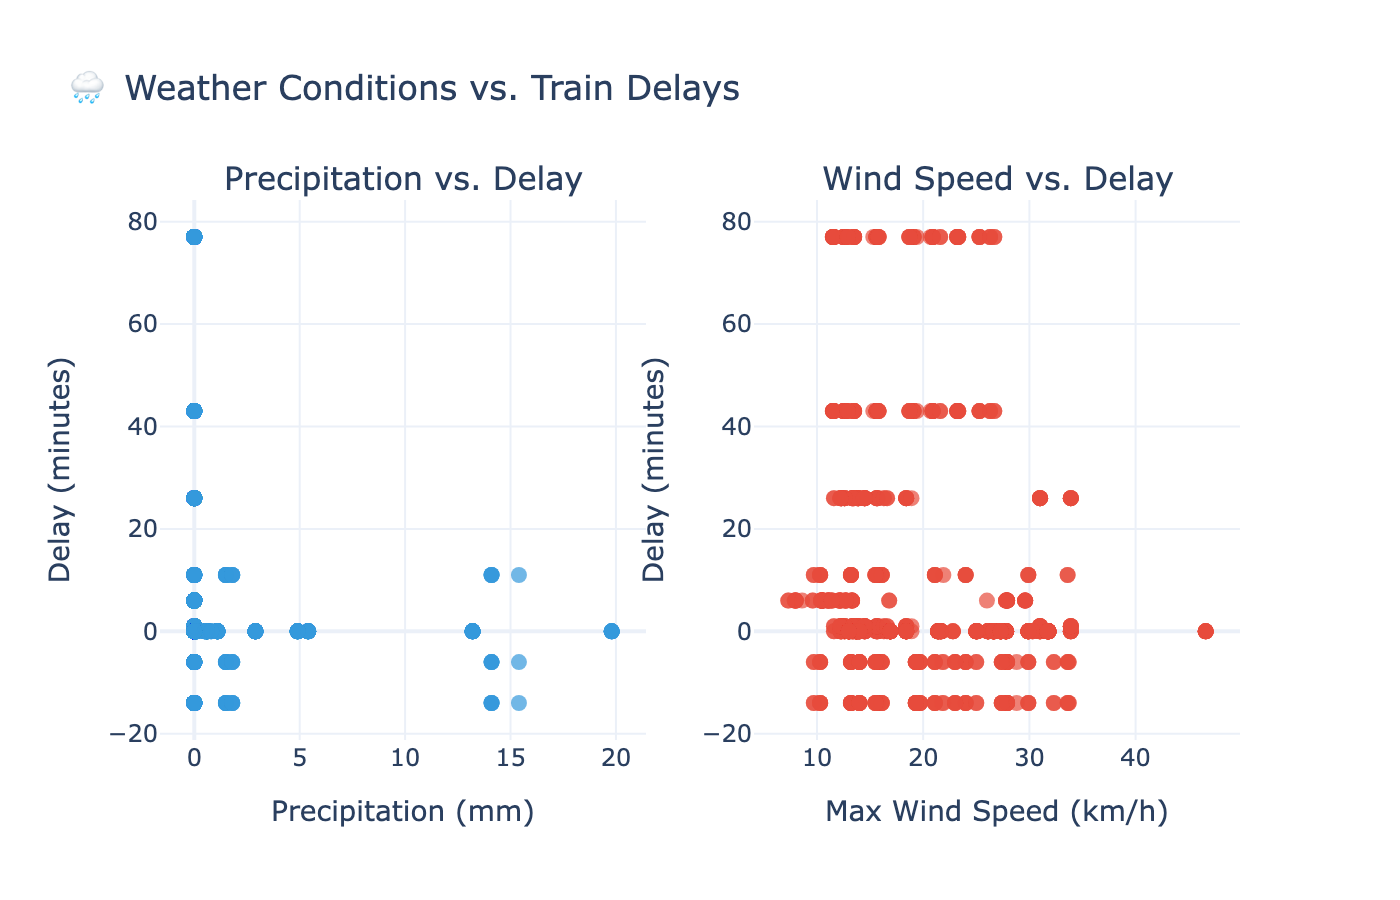
\includegraphics[width=0.55\textwidth]{weather_conditions.png}
    \caption{Scatter plot showing delay distribution across precipitation and maximum wind speed}
    \label{fig:scatter}
\end{figure}


\subsubsection{Correlation Verification}
Running the Pearson and Spearman Correlation tests, it reveals a statistically significant but weak correlation between delays and environmental factors. ($p$-value $\approx 0.001$). Maximum temperature and delays show a positive correlation (Pearson $r \approx +0.26$, Spearman $\rho \approx +0.39$), and precipitation and maximum wind speed show negative correlation with train delays ($r \approx -0.15$ and $-0.18$, respectively). Though weather shows a measurable impact on train delays, it is not significant enough to derive a conclusion. 

\begin{table}[H]
    \centering
    \caption{Pearson and Spearman Correlation Analysis ($N = 1000$)}
    \vspace{0.2cm}
    \begin{tabular}{@{}lccc@{}}
        \toprule
        \textbf{Meteorological Feature} & \textbf{Pearson $r$} & \textbf{Spearman $\rho$} & \textbf{$p$-value} \\
        \midrule
        Precipitation (mm) & $-0.1497$ & $-0.2865$ & $< 0.001$ \\
        Max Wind Speed (km/h) & $-0.1791$ & $-0.2784$ & $< 0.001$ \\
        Max Temperature ($^\circ$C) & $+0.2631$ & $+0.3885$ & $< 0.001$ \\
        \bottomrule
    \end{tabular}
    \label{tab:correlation_stats}
\end{table} 

\begin{figure}[H]
    \centering
    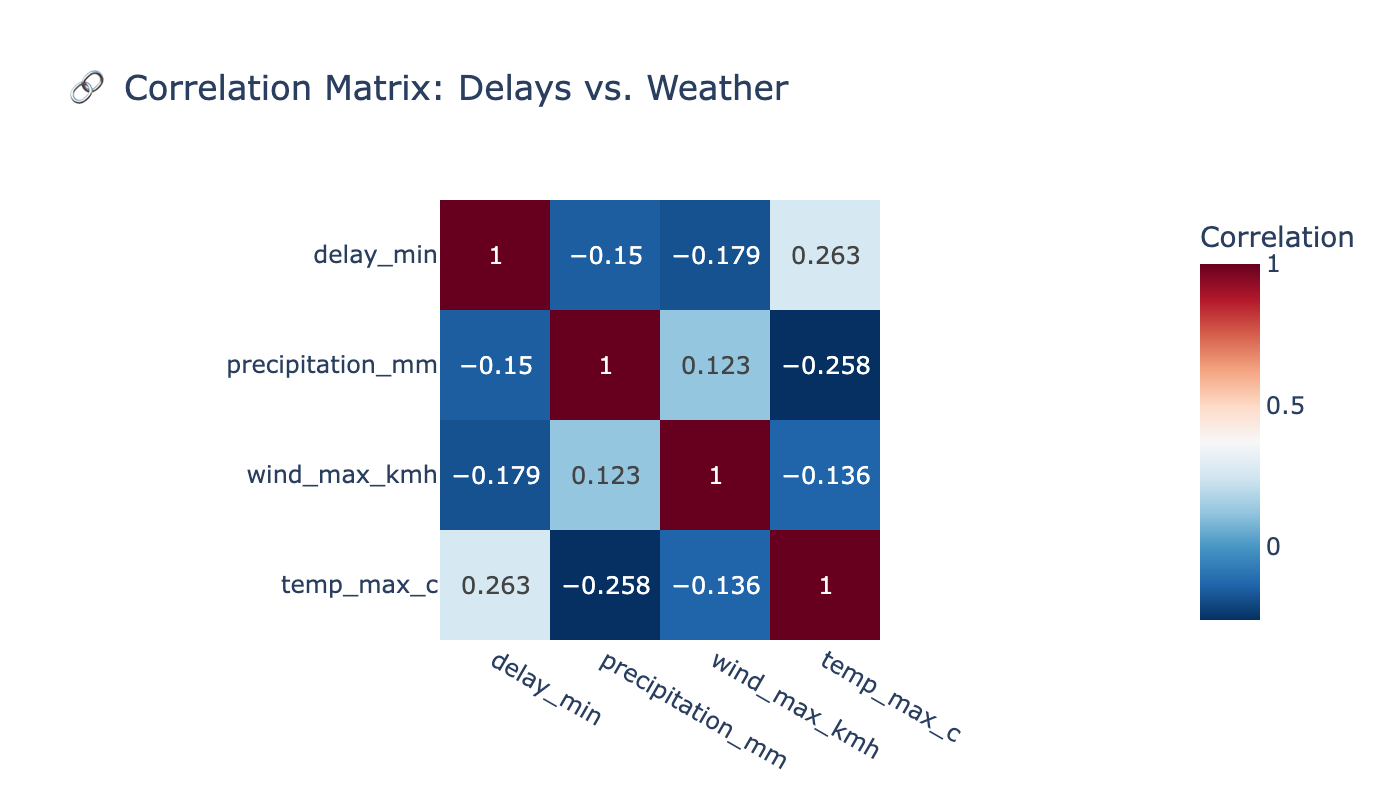
\includegraphics[width=0.65\textwidth]{correlation_matrix.png}
    \caption{Correlation matrix between delays and weather conditions.}
    \label{fig:correlation}
\end{figure}

\subsection{Machine Learning Predictions}

\subsubsection{Model Validation and Accuracy}
The Amtraker website doesn't do any delay predictions, so we thought adding it would give users an idea about delays in particular Amtrak stations, and they can be prepared accordingly. We train two ensemble models: \textbf{Random Forest} and \textbf{Gradient Boosting}. Both models use the same seven features, which are the route name, station name, hour of the day, day-of-week, weekend flag, stop number along the route, and train speed, and were evaluated on the same number of training and testing samples to get a accurate comparison.
\begin{table}[H]
    \centering
    \caption{Model Comparison: Random Forest vs Gradient Boosting}
    \vspace{0.2cm}
    \begin{tabular}{@{}lcc@{}}
        \toprule
        	\textbf{Metric} & \textbf{Random Forest} & \textbf{Gradient Boosting} \\
        \midrule
        Training Samples & 816,995 & 816,995 \\
        Test Samples & 204,249 & 204,249 \\
        MAE & 7.99 minutes & 15.13 minutes \\
        RMSE & 17.95 minutes & 26.56 minutes\\
        $R^2$ & 0.78 & 0.53 \\
        \bottomrule
    \end{tabular}
    \label{tab:metrics}
\end{table}

On the testing data, \textbf{Random Forest performed better}, so we used the Random Forest model for future predictive analysis.
\subsubsection{Feature Importance and Route-Level Interpretation}
The Random Forest model calculates the feature importance based on which internal tree node leads to the final prediction. This analysis confirms that \texttt{Route} and \texttt{Stop \# Along Route} are the most important predictors. This shows that delays are route-driven and can be attributed to various attributes like congestion with a route, the terrain of the route.

\begin{figure}[H]
    \centering
    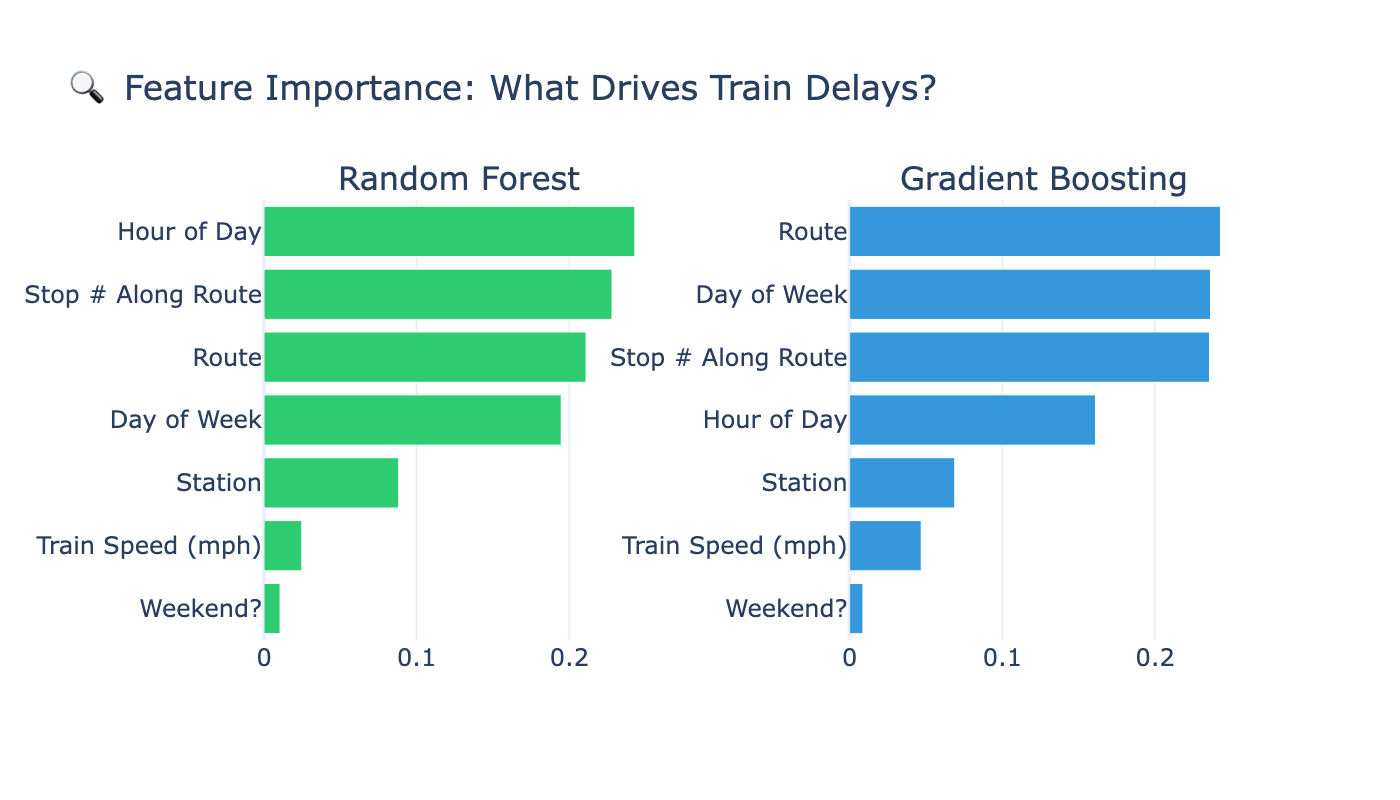
\includegraphics[width=0.6\textwidth]{feature_importance.png}
    \caption{Feature level importance for both Random Forest and Gradient Boosting models}
    \label{fig:route_context_ml}
\end{figure}
As shown in Figure \ref{fig:pred_v_actual}, the models' predictions cluster closely along the red line, which is y=x, which represents perfect predictions. While there can be some predictions that are off, it happens in extreme outliers where the delay is exceeding 200 minutes; this linear agreement shows the model's high forecasting ability due to the ($R^2 = 0.78$) we get.
\begin{figure}[H]
    \centering
    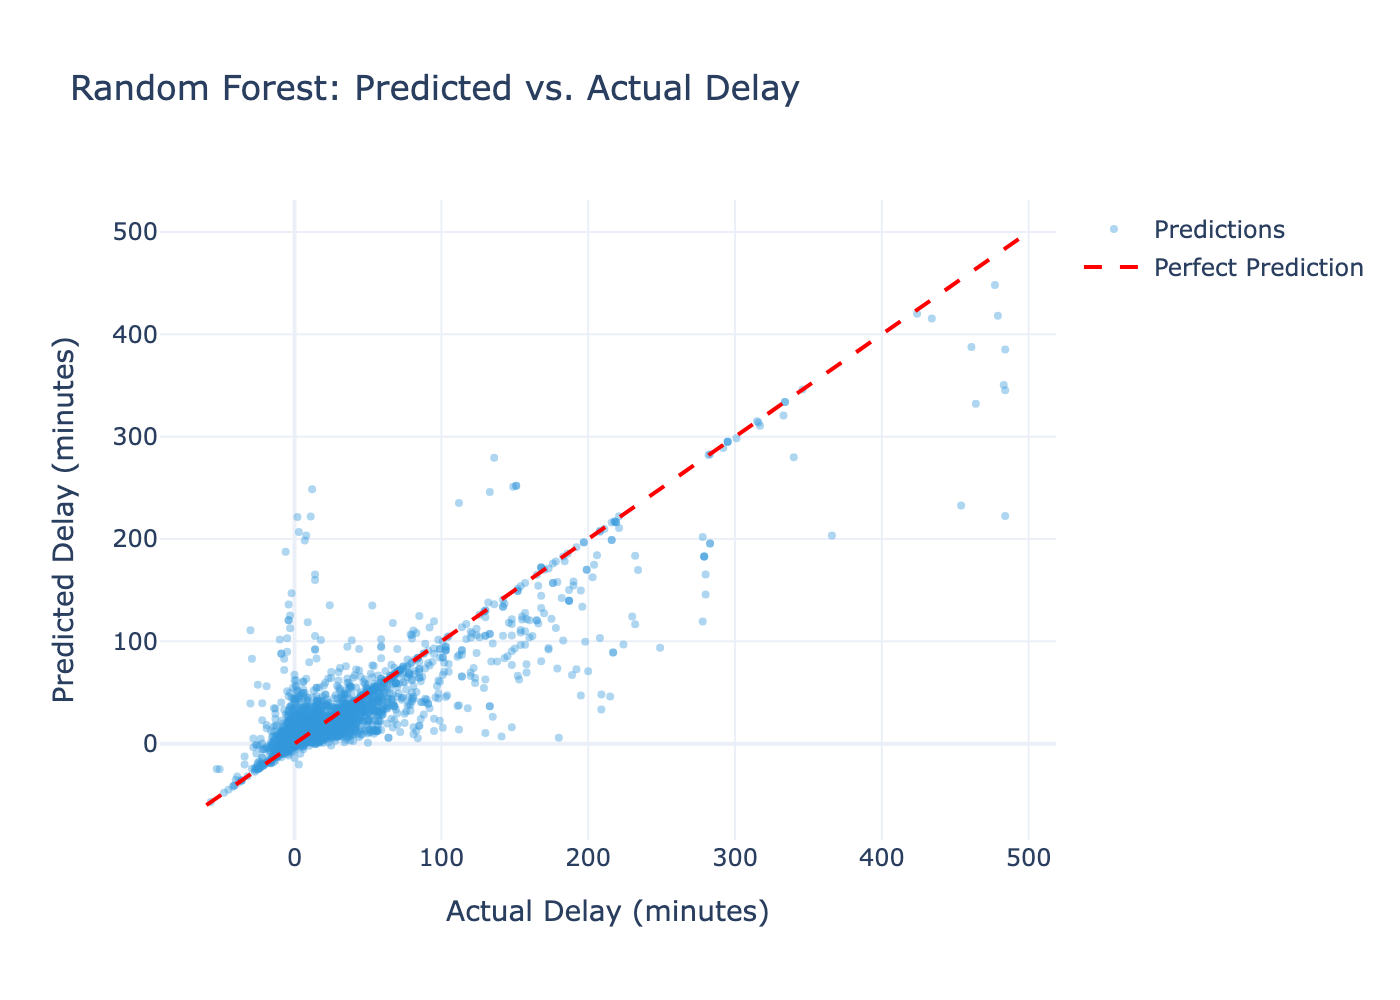
\includegraphics[width=0.6\textwidth]{rf_predicted_vs_actual.png}
    \caption{Predicted vs actual delay, it shows a linear pattern without overfitting}
    \label{fig:pred_v_actual}
\end{figure}

As shown in Figure \ref{fig:predictions}, the model is able to predict the delays accurately. It is able to capture very high positive delays in the case of Empire Builder, and even when the trains are arriving before the scheduled arrival in the case of Auto Train.
\begin{figure}[H]
    \centering
    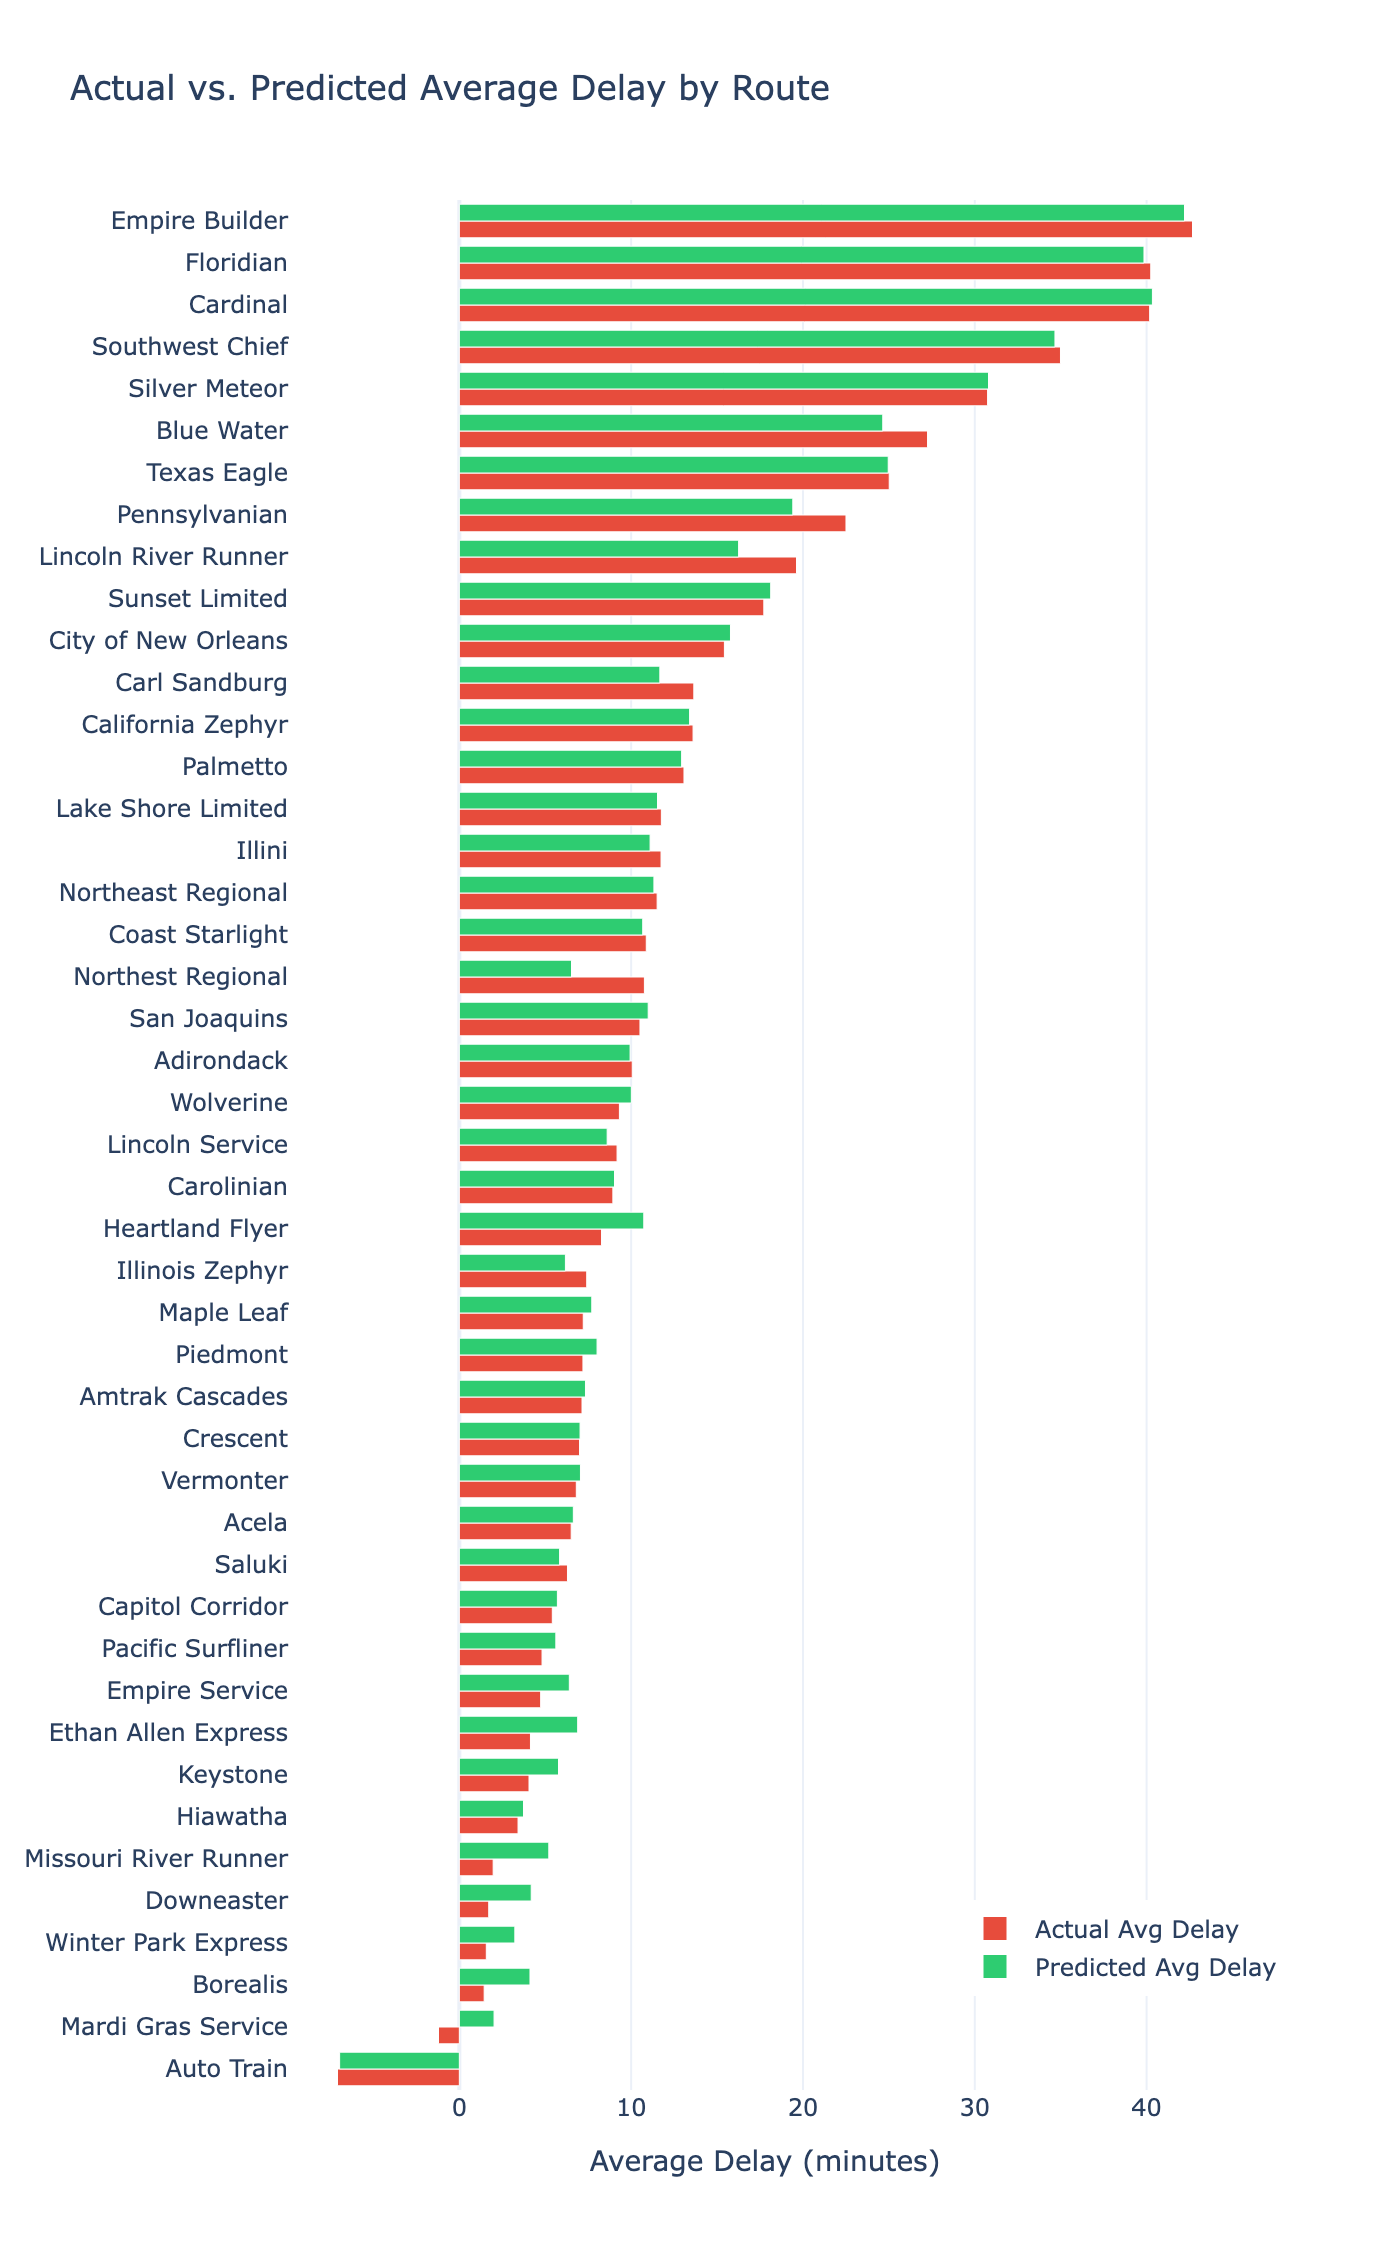
\includegraphics[width=0.6\textwidth]{route_actual_vs_predicted.png}
    \caption{Plot showing the predicted vs actual delays across routes}
    \label{fig:predictions}
\end{figure}

\section{Summary / Conclusion}

\subsection{What we found}
We built an automated system that scrapes live Amtrak data, run statistical tests on it, and trains a machine learning model on the results. The ANOVA and correlation results were pretty clear: extreme delays track with route infrastructure (the specific line, the stop number, train speed) far more than with local weather conditions. While Feeding those infrastructure variables into a Random Forest model, we got delay predictions within about 7 minutes of actual outcomes.






\subsection{Project Limitations}
While algorithmically sound, explicit engineering constraints temper conclusions regarding broader macro-applicability:
\begin{itemize}
    \item \textbf{Short Window for data collection:} We only had about 10 days of live data. That’s enough to spot route-level patterns, but not nearly enough for seasonal ones. The model knows nothing about winter freeze.
    \item \textbf{Geographic Weather Abstraction:} Weather data was limited to 10 major station hubs because of API rate limits. This is a real blind spot. A train can run through a blizzard in rural Iowa while the Chicago hub reports clear skies, and our data would only see the clear skies.
    \item \textbf{Hidden Root Causes:} The delay data also lacks any causal information. The APIs report duration but not the reason. This is a mechanical failure and a freight bottleneck produce identical records. That noise is sitting in the residuals, and we can’t separate it.
\end{itemize}

\subsection{Future Directions}
The scraper needs to run for a full year. Ten days got us this far, but 12 months of data (roughly 70 million records) would let the model pick up seasonal trends. Another improvement worth pursuing is GPS-based weather lookup. This would pull conditions at the train’s actual coordinates instead of the nearest hub station. That would go a long way toward clarifying whether weather matters more than our current data suggests.

\vspace{1cm}
\renewcommand{\refname}{}
\section{References}
\vspace{-1.5cm}
\begin{thebibliography}{9}
    \bibitem{ref:amtraker} Amtraker User API v3 Repository and Endpoints. Available online: \url{https://api-v3.amtraker.com/}
    \bibitem{ref:meteo} Open-Meteo Historical open-source Meteorological API. Available online: \url{https://open-meteo.com/}
    \bibitem{ref:wiki} \textit{List of Amtrak Stations}. Wikipedia, The Free Encyclopedia. Available online: \url{https://en.wikipedia.org/wiki/List_of_Amtrak_stations}
\end{thebibliography}

\clearpage
\renewcommand{\listfigurename}{}
\renewcommand{\listtablename}{}
\section{List of Figures and Tables}
\vspace{-1.5cm}
\listoffigures
\vspace{0.5cm}
\listoftables

\section*{Appendix: Code Implementation}
\addcontentsline{toc}{section}{Appendix: Code Implementation}

This appendix describes the key components of our python data engineering framework and how we capture, confirm the time and commit to our relational schemas.


\subsection*{A.1:  Delay Data Parsing}
The target variables will not be correctly computed unless we resolve the issues of which timestamps NaN and which are consistent with the ISO 8601 timestamp standard.


\begin{lstlisting}[language=Python, caption=Parsing and executing chronological metrics natively via datetime libraries.]
from datetime import datetime

def parse_delay_minutes(scheduled, actual):
    """Calculate delay in minutes between scheduled and actual times."""
    if not scheduled or not actual:
        return None
    try:
        sch = datetime.fromisoformat(scheduled)
        act = datetime.fromisoformat(actual)
        delta = (act - sch).total_seconds() / 60.0
        return round(delta, 1)
    except (ValueError, TypeError):
        return None
\end{lstlisting}

\subsection*{A.2: Active Training Pipeline (Random Forest)}
Identify how we can determine an evaluation architecture and how to evaluate error margins against the actual real-time array.


\begin{lstlisting}[language=Python, caption=Machine Learning feature initialization mapping encoded integers to regression arrays.]
import numpy as np
from sklearn.ensemble import RandomForestRegressor
from sklearn.model_selection import train_test_split

# Defining strictly continuous and categorical encoded features
features = [
    'route_encoded', 
    'station_encoded', 
    'hour', 
    'day_of_week', 
    'is_weekend', 
    'stop_number', 
    'velocity'
]
X = df_cleaned[features]
y = df_cleaned['delay_arrival_min']

# Partitioning Matrix uniformly 
X_train, X_test, y_train, y_test = train_test_split(
    X, y, test_size=0.2, random_state=42
)

# Initialize optimized Random Forest Regressor resolving nonlinear cascades
rf_model = RandomForestRegressor(
    n_estimators=100, 
    max_depth=20, 
    min_samples_split=5,
    random_state=42,
    n_jobs=-1
)

rf_model.fit(X_train, y_train)
predictions = rf_model.predict(X_test)
\end{lstlisting}
\end{lstlisting}

\subsection*{A.3: Resolving Zero Variance Issues in Weather DataFrames}
During the exploratory data analysis conducted early in the process, zero variance standard errors were produced from all correlation computations between extreme delays and various weather-related data. The source of this issue is due to the limitation placed on the SQL JOIN clause for the two tables during data extraction; specifically, the final sample of information extracted included only the most extreme delays (listed via ORDER BY delay arrival minutes DES LIMIT 30). As a result of this extraction process, the sample included only the network's most significant bottleneck, i.e., all delays greater than 300 minutes or greater in delay. When evaluating and computing linear correlation using zero variance, the mathematics of division generate a crash of the correlation computation. Therefore, by removing the limit of examining only extreme delay times and evaluating the entire cross-section of daily transit time frames provides the necessary basis for confirming the minimal impact weather has had on overall delay variance and how to calculate correlations of the two variables in a statistically valid manner.

\begin{lstlisting}[language=SQL, caption=Corrected SQL logic omitting extreme outliers to establish true network-wide weather associations.]
-- Original Problematic Query Constraint (Created NaN errors due to Zero Variance)
-- ORDER BY d.delay_arrival_min DESC
-- LIMIT 30

-- Corrected Query resolving natural meteorological distribution
query3 = """
    SELECT 
        d.route_name,
        d.station_code,
        d.station_name,
        ROUND(d.delay_arrival_min, 1) as delay_min,
        w.temp_max_c,
        w.precipitation_mm,
        w.wind_max_kmh,
        w.weather_code
    FROM delay_logs d
    INNER JOIN weather w 
        ON d.station_code = w.station_code
    WHERE d.delay_arrival_min IS NOT NULL
      AND d.status = 'Departed'
    -- Limit expanded substantially without forced descending sort
    LIMIT 1000  
"""
df_q3 = pd.read_sql_query(query3, conn)
\end{lstlisting}


\end{document}